% !TEX root = ~/base_de_donnee/LETEX.tex
\documentclass{report}


\usepackage[utf8]{inputenc}
\usepackage[T1]{fontenc}
\usepackage[francais]{babel}
\usepackage{pdfpages}
\usepackage{supertabular}

\begin{document}

\part{Projet BDD : Forum nouvelles technologies}
\chapter{Presentation du projet}
\section{Description du projet}



Le forum “le E-forum” propose les services suivants:
création d'utilisateur
\begin{itemize}
\item modification d’un profil d’utilisateur
\item un utilisateur peut poster et lire des messages
\item un message est contenu dans une unique catégorie
\item proposition de profil pour recruteur
\end{itemize}

\section{Description des entités:}
Utilisateur:
\begin{itemize}
		\item Pseudonyme
		\item Adresse Mail
		\item Date Naissance
		\item Sexe
		\item Ville
		\item Etude
		\item Nombre de message
		\item Moyenne de la qualité des messages
		\item Statut de l'utilisateur (Recruteur/modérateur/administrateur/lambda/utilisateur supprimé)
		\item Date de dernière connexion\\
\end{itemize}
Message:
\begin{itemize}
	\item Id message
	\item Date du message
	\item Contenu du message
	\item Qualité du message\\
\end{itemize}
\pagebreak
Catégorie
\begin{itemize}
	\item Nom de la catégorie
	\item Popularité\\
\end{itemize}
Sujet
\begin{itemize}
	\item Id sujet
   \item Nom sujet
	\item Date de creation du sujet
	\item Popularité du sujet\\
\end{itemize}
	Support
  \begin{itemize}
		\item ID du support
		\item Système d’exploitation
		\item Navigateur internet\\
  \end{itemize}
	Rang
  \begin{itemize}
		\item Nom du rang
		\item Palier d'accès\\
    \end{itemize}
	Statistiques
  \begin{itemize}
		\item Date
		\item Tranche Horaire
		\item Nombre de connexions
		\item Nombre de message postés\\
    \end{itemize}
	Section
  \begin{itemize}
		\item Nom Section
		\item Popularité Section\\
  \end{itemize}
	Offre Recrutement
	\begin{itemize}
	\item Id Annonce
	\item Date butoire
	\item Date Annonce
	\item Type Annonce
	\item Type Contrat
	\item Message de l'annonce\\
	\end{itemize}
	Message privé
	\begin{itemize}
	\item ID message privé
	\item Date MP
	\item Contenu MP
	\item Etat MP (lu/ non lu)\\
	\end{itemize}
	Programmation
	\begin{itemize}
	\item Langage programmation\\
	\end{itemize}

\section{Description des fonctionnalités:}

\subsection{Création d'un utilisateur}
		Il doit remplir les champs suivant : nom, prénom, date 	de naissance, sexe, ville, adresse mail, langage de programmation et son niveau et ou domaine d’étude ainsi que sa disponibilité au recrutement pour un ou des langage(s).

\subsection{Modification d’un utilisateur}
		Tous les utilisateurs peuvent changer leurs informations 	suivantes : ville , études, langage de programmation, niveau 	de programmation. Il peut également modifier ses disponibilités en rapport au recrutement.

\subsection{Suppression d’un utilisateur}
		Si un utilisateur décide de supprimer son compte, on 	conserve le profil mais il passe dans la liste des 	utilisateurs 	supprimés. Ses messages restent disponibles mais le 	pseudo 	passe en «compte supprimé». Le pseudo d'origine ne 	sera pas 	réutilisable par d'autres utilisateurs.
\subsection{Droit des utilisateurs}
		Un utilisateur normal peut poster des messages et    	créer des sujets. Il peut supprimer ses propres messages et 	fermer ses propres sujets.\\
		Un modérateur est responsable d’une ou plusieurs 	catégorie(s). Il peut modifier et supprimer les 			messages et les sujets des autres utilisateurs et 			promouvoir des utilisateurs au status de recruteur.\\
		Un administrateur possède les mêmes droits qu'un 	modérateur mais il peut aussi consulter les stats du 		forum, ainsi que supprimer des utilisateurs.
		Un recruteur acquiert son status après demande à un 	administrateur ou modérateur. Il dispose des mêmes 	droits 	qu'un utilisateur normal mais dispose en plus d'un accès à un 	outil de recherche de candidats potentiels.\\

\subsection{Proposition de profil pour recruteur}
		Un recruteur peut demander certaines conditions 	lors de sa recherche de candidats: un périmètre de 		recherche, âge, sexe, études, langage et le serveur lui 	retournera une liste de 5 profils correspondant au mieux à sa 	recherche.\\
	\pagebreak	
\subsection{Offres de recrutement}
Les recruteurs peuvent déposer des offres de recrutement en spécifiant une date limite, le type de contrat offert(CDD, CDI, Stage, Alternance), le type de l'annonce (WEB, Logiciels, hardware...). Il peut également spécifier les qualifications nécessaires.\\

\subsection{Structure du forum}
		Le forum est composé de plusieurs sections fixées 	par les administrateurs. (ex:  Informatique, Jeux Vidéos, 	Sciences, Bric-à-Brac …).\\
		Ces sections sont composées de catégories, elles 	aussi créées par les administrateurs. Une catégorie 		possède un unique modérateur. (ex: Pour la section 		Informatique, on pourrait retrouver des catégories telles 	que:  Programmation, Matériel, Demande d'aides …).\\
		Dans les catégories, les utilisateurs peuvent créer 	des sujets ainsi que poster des messages dans leurs 		sujets et dans les sujets d'autres utilisateurs.\\
		Les différents éléments présentés ci-dessus auront 	une note de «qualité», présentée ci-dessous.\\
\subsection{Messages privés}
Les utilisateurs peuvent échanger des messages privés. Un message privé ne possède qu'un seul destinataire. L'utilisateur ayant envoyé le message sait si ce dernier est lu ou pas.

\subsection{Statistiques d’utilisation du forum}
		A chaque message posté par un utilisateur, son nombre 	de messages s'incrémente.\\
		Lorsqu'un message est vu, le compteur de popularité 	correspondant à sa catégorie et sa section augmente de 0.01.\\
		A chaque «upvote» sur un message, sa qualité augmente 	de 1.\\
		A chaque «downvote» sur un message, sa qualité 	diminue de 0,5.\\
		Une moyenne sera calculée pour chaque utilisateur selon 	la qualité de ses messages.
		Tous les jours à minuit, le serveur, pour chaque 	personne, va calculer sa moyenne de qualité et va lui définir 	un rang.\\
		Il va aussi calculer le nombre de message sur la journée 	dans chaque section/catégorie, les périodes de fréquentation, 	la proportion d'âge par catégorie, les préférences de langage 	et le sexe par catégorie.\\
		De plus, à chaque connexion/déconnexion, un “tableau” 	de connexion est mis à jour et à minuit le serveur définit les 	plages horaires où le forum a été le plus actif / inactif et reset 	le tableau.
		A chaque connexion, le serveur détermine le support de 	l’utilisateur.\\

\chapter{Conception du projet}
\section{Matrice des DF}
\begin{supertabular}{|c|c|c|c|c|c|c|c|c|c|c|c|c|c|c|c|}
\hline
A->B &  & 1 & 12 & 16 & 18 & 22 & 25 & 27 & 31 & 32 & 9 & 9+1 & 36 & 39 & 36+9 \\
\hline
1 & Pseudo & x & x &  & x & x &  &  &  &  &  &  & x & x & \\
\hline
2 & AdresseMail & x & x &  & x & x &  &  &  &  &  &  & x & x & \\
\hline
3 & DateNaissance & x & x &  & x & x &  &  &  &  &  &  & x & x & \\
\hline
4 & Sexe & x & x &  & x & x &  &  &  &  &  &  & x & x &  \\
\hline
5 & Ville & x & x &  & x & x &  &  &  &  &  &  & x & x & \\
\hline
6 & Etude & x & x &  & x & x &  &  &  &  &  &  & x & x & \\
\hline
7 & NbMessage & x & x &  & x & x &  &  &  &  &  &  & x & x & \\
\hline
8 & MoyQualitéMsg & x & x &  & x & x &  &  &  &  &  &  & x & x & \\
\hline
9 & LangageProg &  &  &  &  &  &  &  &  &  & x &  & x &  & \\
\hline
10 & NiveauProg &  &  &  &  &  &  &  &  &  &  & x &  &  & x\\
\hline
11 & DateDerniereConnection & x & x &  & x & x &  &  &  &  &  &  & x & x & \\
\hline
12 & IdMsg &  & x &  &  &  &  &  &  &  &  &  &  &  & \\
\hline
13 & DateMsg &  & x &  &  &  &  &  &  &  &  &  &  &  &   \\
\hline
14 & ContenuMsg &  & x &  &  &  &  &  &  &  &  &  &  &  & \\
\hline
15 & QualitéMsg &  & x &  &  &  &  &  &  &  &  &  &  &  &  \\
\hline
16 & NomCatégorie &  & x & x & x &  &  &  &  &  &  &  &  &  & \\
\hline
17 & PopularitéCatégorie &  & x & x & x &  &  &  &  &  &  &  &  &  & \\
\hline
18 & IdSujet &  & x &  & x &  &  &  &  &  &  &  &  &  & \\
\hline
19 & NomSujet &  & x &  & x &  &  &  &  &  &  &  &  &  & \\
\hline
20 & DateCreationSujet &  & x &  & x &  &  &  &  &  &  &  &  &  & \\
\hline
21 & PopularitéSujet &  & x &  & x &  &  &  &  &  &  &  &  &  & \\
\hline
22 & IdSupport &  &  &  &  & x &  &  &  &  &  &  &  &  & \\
\hline
23 & SystemeExploitation &  &  &  &  & x &  &  &  &  &  &  &  &  & \\
\hline
24 & NavigateurInternet &  &  &  &  & x &  &  &  &  &  &  &  &  & \\
\hline
25 & NomRang & x & x &  & x & x & x &  &  &  &  &  & x & x & \\
\hline
26 & PalierAcces & x & x &  & x & x & x &  &  &  &  &  & x & x & \\
\hline
27 & Date &  &  &  &  &  &  & x &  &  &  &  &  &  & \\
\hline
28 & TrancheHoraire &  &  &  &  &  &  & x &  &  &  &  &  &  & \\
\hline
29 & NombreConnec &  &  &  &  &  &  & x &  &  &  &  &  &  & \\
\hline
30 & NombreMsgPostés &  &  &  &  &  &  & x &  &  &  &  &  &  & \\
\hline
31 & IntituléStatus & x & x &  & x & x &  &  & x &  &  &  & x & x & \\
\hline
32 & NomSection &  & x & x & x &  &  &  &  & x &  &  &  &  & \\
\hline
33 & PopularitéSection &  & x & x & x &  &  &  &  & x &  &  &  &  & \\
\hline
34 & DateAnnonce &  &  &  &  &  &  &  &  &  &  &  & x &  & \\
\hline
35 & DateButoire &  &  &  &  &  &  &  &  &  &  &  & x &  & \\
\hline
36 & IdAnnonce &  &  &  &  &  &  &  &  &  &  &  & x &  & \\
\hline
37 & TypeAnnonce &  &  &  &  &  &  &  &  &  &  &  & x &  & \\
\hline
38 & MsgAnnonce &  &  &  &  &  &  &  &  &  &  &  & x &  & \\
\hline
39 & IdMP &  &  &  &  &  &  &  &  &  &  &  &  & x & \\
\hline
40 & DateMP &  &  &  &  &  &  &  &  &  &  &  &  & x  & \\
\hline
41 & ContenuMP &  &  &  &  &  &  &  &  &  &  &  &  & x & \\
\hline
42 & EtatMP &  &  &  &  &  &  &  &  &  &  &  &  & x  & \\
\hline
43 & DispoRct &  &  &  &  &  &  &  &  &  &   & x &  &  & \\
\hline
\end{supertabular}
\section{Listes des transitions simplifié des DF}
\begin{supertabular}{|c|c|c|c|c|c|c|c|c|c|c|}
\hline
1>2 & 12>1 & 16>17 & 18>1 & 22>1 & 25>26 & 27>28 & 32>33 & 9>10 & 36>1 & 39>1\\
\hline
1>3 & 12>13 & 16>32 & 18>16 & 22>23 &  & 27>29 &  & & 36>34 & 39>40\\
\hline
1>4 & 12>14 &  & 18>19 & 22>24 &  & 27>30 &  &  & 36>35 & 39>41\\
\hline
1>5 & 12>15 &  & 18>20 &  &  &  &  &  & 36>37 & 39>42\\
\hline
1>6 & 12>18 &  & 18>21 &  &  &  &  &  & 36>38 & \\
\hline
1>7 & &  & 18>33 &  &  &  &  &  &  & \\
\hline
1>8 &  &  &  &  &  &  &  &  &  & \\
\hline
1>11 &  &  &  &  &  &  &  &  &  & \\
\hline
1>25 &  &  &  &  &  &  &  &  &  & \\
\hline
1>31 &  &  &  &  &  &  &  &  &  & \\
\hline
\end{supertabular}
9+1>10\\
36+1>10
\newpage
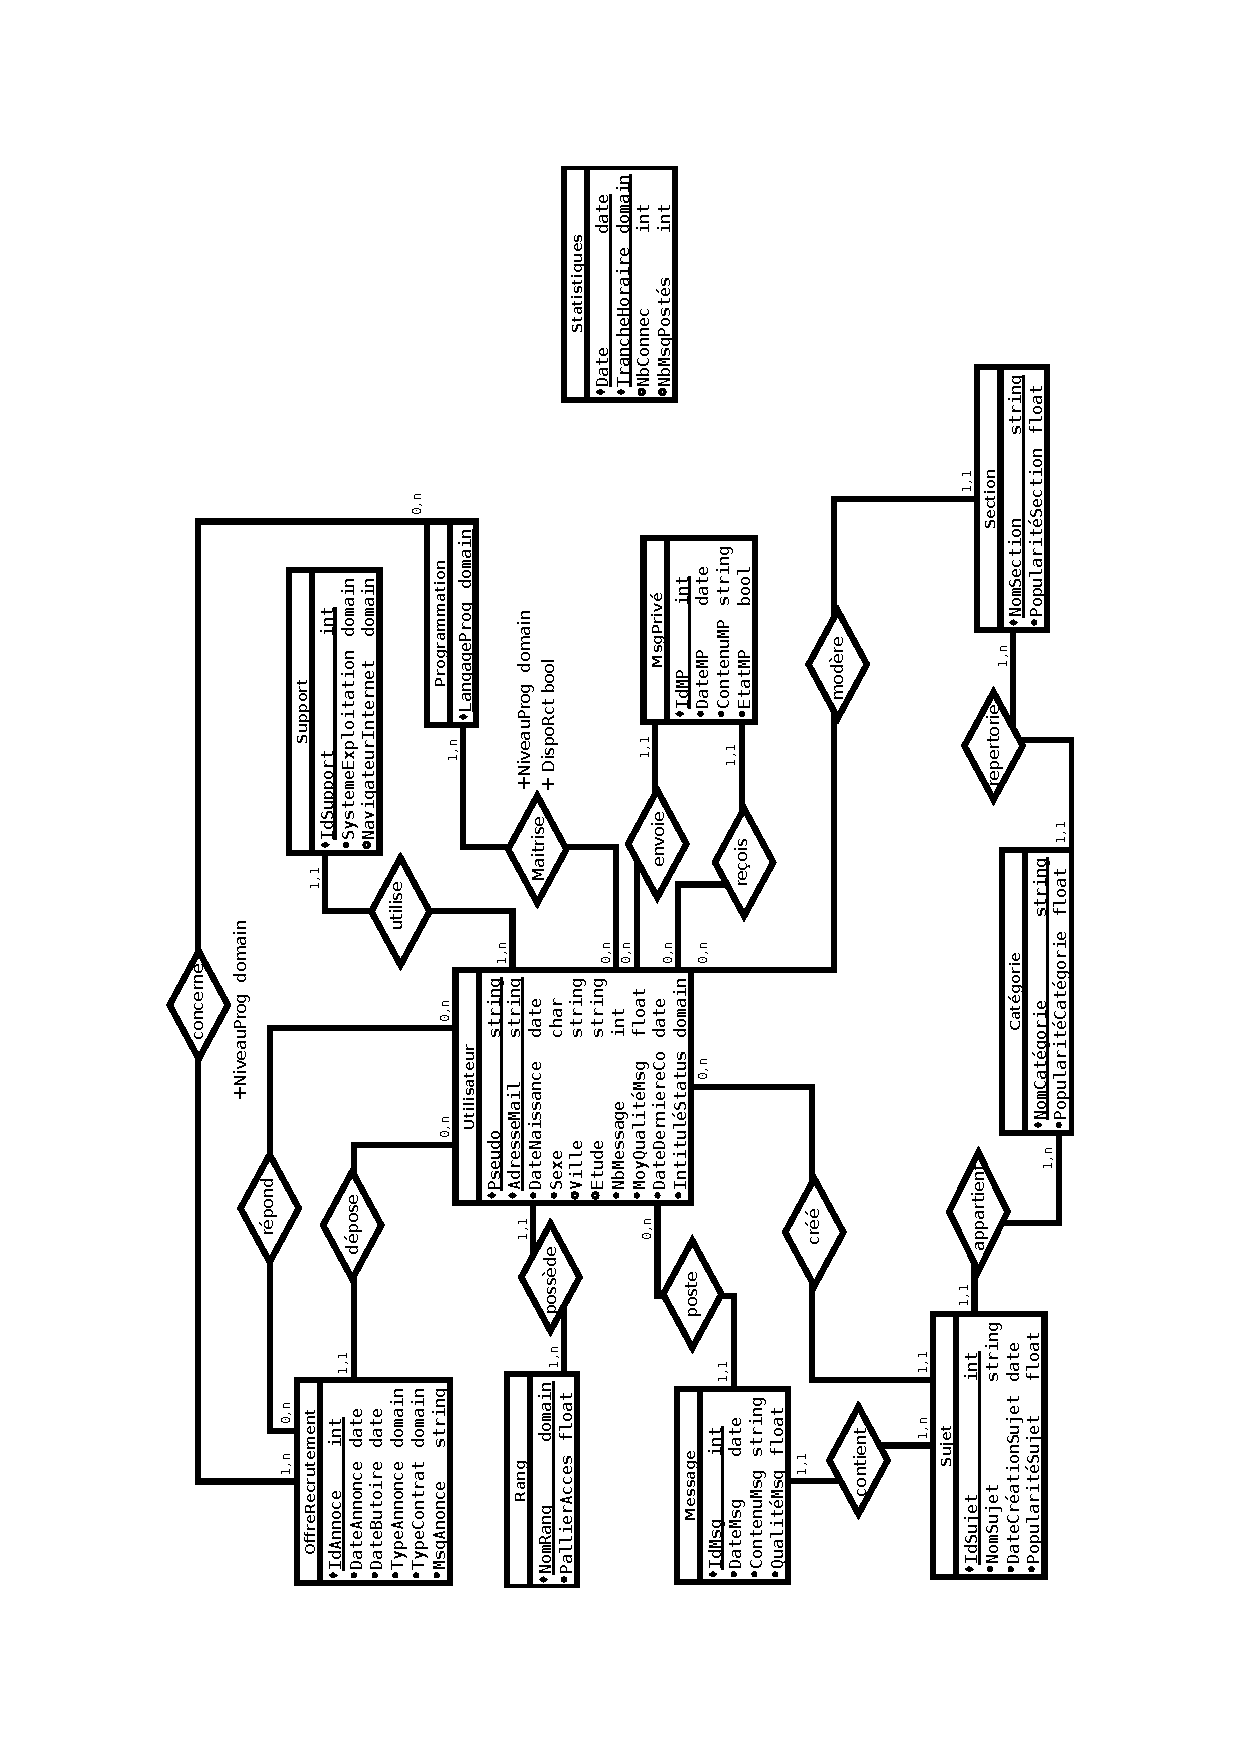
\includepdf[pages={1},angle=270,pagecommand=\section{Mea}]{MEA.pdf}
\section{Modele}
utilisateur(\underline{Pseudo}, \underline{AdresseMel}, DateNaissance, Sexe, Ville, Etude, nbMessage, MoyenneQualitéMsg, DerniereConnexion, \#NomRang, IntituleStatus)\\

Message(\underline{IdMessage}, DateMessage, Contenu, QualitéMsg, \#Pseudo, \#IdSujet)\\

Sujet(\underline{IdSujet}, NomSujet, DateCreation, PopularitéSujet, \#NomCategorie, \#Pseudo)\\

Catégorie(\underline{NomCategorie}, popularitéCatégorie, \#NomSection)\\

Section(\underline{NomSection}, PopularitéSection, \#Moderateur)\\

Rang(\underline{NomRang}, PalierAcces)\\

Support(\underline{Idsupport}, systemeExploitation, NavigateurWeb, \#Pseudo)\\

Statistiques(\underline{Date}, \underline{TrancheHoraire}, NbConnections, NbMessagesPostés)\\


Offrerecrutement(\underline{IdAnnonce}, DateAnnonce, DateButoire, TypeAnnonce, TypeContrat, MsgAnnonce, \#Pseudo)\\

Msgprive(\underline{IdMP}, DateMP, ContenuMp, EtatMp, \#pseudo-envoi, \#pseudo-recoit)\\

Programmation(\underline{LangageProg})\\

utilisateurProgrammation(\underline{\#pseudo},\underline{\#langageProg}, NiveauProg, DispoRct)\\

offreRecrutementProgrammation(\underline{\#Idannonce},\underline{\#langageProg}, NiveauDemande)\\

UtilisateurOffreRecrutement(\underline{\#IdAnnonce}, \underline{\#Pseudo})

\chapter{Fonctionnalités proposé au niveau de la bdd}
\section{Requetes}
Diverses requêtes seront proposées:\\
 - Affichage du nombre total de messages;\\
 - Affichage du nombre total d’utilisateurs;\\
 - Affichage de tous les messages d'un utilisateur;\\
 - Affichage de tous les messages d'un utilisateur dans une tranche horaire;\\
 - Affichage de tous les messages d'un sujet;\\
 - Affichage de tous les messages privés d'une personne;\\
 - Affichage de tous les messages privés provenant d'une certaine personne;\\
 - Affichage des proportions des systèmes d'exploitations utilisés;\\
 - Affichage des proportions des navigateurs internet utilisés;\\
 - Nombre de connexions tranche horaire;\\
 - Nombre de connexions par date;\\
 - Nombre de messages postés par tranche horaire;\\
 - Nombre de messages postés par dates;\\
 - Nombre de candidats possible pour un recruteur;\\
 - Nombre de comptes par villes;\\
 - Tranche d’age des utilisateurs;\\
 - Liste de messages contenant un motif;\\
 - Recherche de profil en fonction du niveau et type de programmation;\\
 - Recherche d'un profil en fonction d'un pseudo;\\
 - Nombre de messages par catégorie;\\
 - Nombre de sujet par catégorie;\\
 - Affichage toutes les annonces en fonction du langage/type contrat;\\
\section{Triggers}
Des triggers pourront être mis en place:\\
 - Insertion/modification/suppression d'un message => modification de la moyennequalitémsg de l'utilisateur concerné;\\
 - Modification à la connexion d'un utilisateur => modification de la stat de connexions par heure et de la date de dernière connexion de l'utilisateur;\\
 - Insertion d'un message => modification de la stat de messages par heure;\\
 - Insertion/suppression d'un message => modification du nombre de message;\\
 - Insertion/modification d'un message => check s'il faut changer de rang;\\
 - Insertion d'un utilisateur => vérification des informations (unicité du pseudo, mail valide);\\
 - Insertion d'une demande de recrutement => vérification de la date limite de dépôt;\\
 - Insertion d'une offre de recrutement => vérification dateButoire > DateAnnonce;\\
 - Modification de modérateur => vérification qu'il n'y a qu'un seul modérateur par section;\\
\section{Vues}
 - Une vue permettant d'accéder au profil les plus favorables pour un recruteur;\\
 - Une vue permettant d'avoir un pack de n messages consécutifs temporellement dans un sujet;\\
 - Une vue permettant d'avoir un pack de n sujets consécutifs temporellement dans une catégorie;
\pagebreak
\section{Roles}
Administrateur:
\begin{itemize}
	\item Un administrateur peut lire et modifier tout les messages postés;
	\item Un administrateur peut accéder à toutes les données et  les modifier de tout les utilisateurs;
	\item Un administrateur peut accéder à toutes les statistiques;\\
\end{itemize}

Modérateur:
\begin{itemize}
	\item Un modérateur peut lire et modifier tout les messages postés sur la section sous sa responsabilité;
  \item Un modérateur peut lire tout les messages du forum;
	\item Un modérateur peut accéder au données public des utilisateurs;\\
\end{itemize}


Recruteur:
\begin{itemize}
  \item Un recruteur peut lire et modifier tout les messages postés par lui même;
  \item Un recruteur peut lire tout les messages du forum;
  \item Un recruteur peut accéder au données public des utilisateurs;\\
\end{itemize}



Utilisateur lambda inscrit:
\begin{itemize}
  \item Un utilisateur lambda inscrit peut lire et modifier tout les messages postés par lui même;
  \item Un utilisateur lambda inscrit peut lire tout les messages du forum;
  \item Un utilisateur lambda inscrit peut accéder au données public des utilisateurs;\\
\end{itemize}


Utilisateur lambda non inscrit:
\begin{itemize}
  \item Un utilisateur lambda non inscrit ne peut pas lire ou modifier aucun messages;
  \item Un utilisateur lambda non inscrit ne peut accéder a aucune information sur les utilisateurs;\\
\end{itemize}

\chapter{Bilan du projet}
Ce projet nous a permis d'apprendre à gérer une base de données et a l'implémenter dans un module internet, d'améliorer nos capacités de gestion du travail en groupe dans un temps limité.\par 
Nous avons pu découvrir d'autres aspects de la programmation, notamment concernant l'aspect web et la gestion de données. 
\end{document}
